\chapter{Evaluation der 3D-Technologien}
\label{CHAP:EVALUATION}

Nachdem das Grundprinzip und die Funktionsweise von WebGL und X3DOM im vorherigen Kapitel ausführlich dargelegt wurden, werden diese im Folgenden anhand der in Kapitel \ref{CHAP:REQUIREMENTS} spezifizierten Kriterien evaluiert.
Hierfür wird zunächst kurz die Testumgebung beschrieben, welche für die Erprobung der Technologien implementiert wurde, und die verwendete Methodik erläutert. Schließlich wird die eigentliche Evaluation mittels verschiedener Tests durchgeführt und die Ergebnisse im Bezug auf die Zielsetzung bewertet.

\section{Architektur der Testumgebung}

\begin{figure}[htb]
	\centering
	\subfloat[Laden eines 3D-Modells]{
		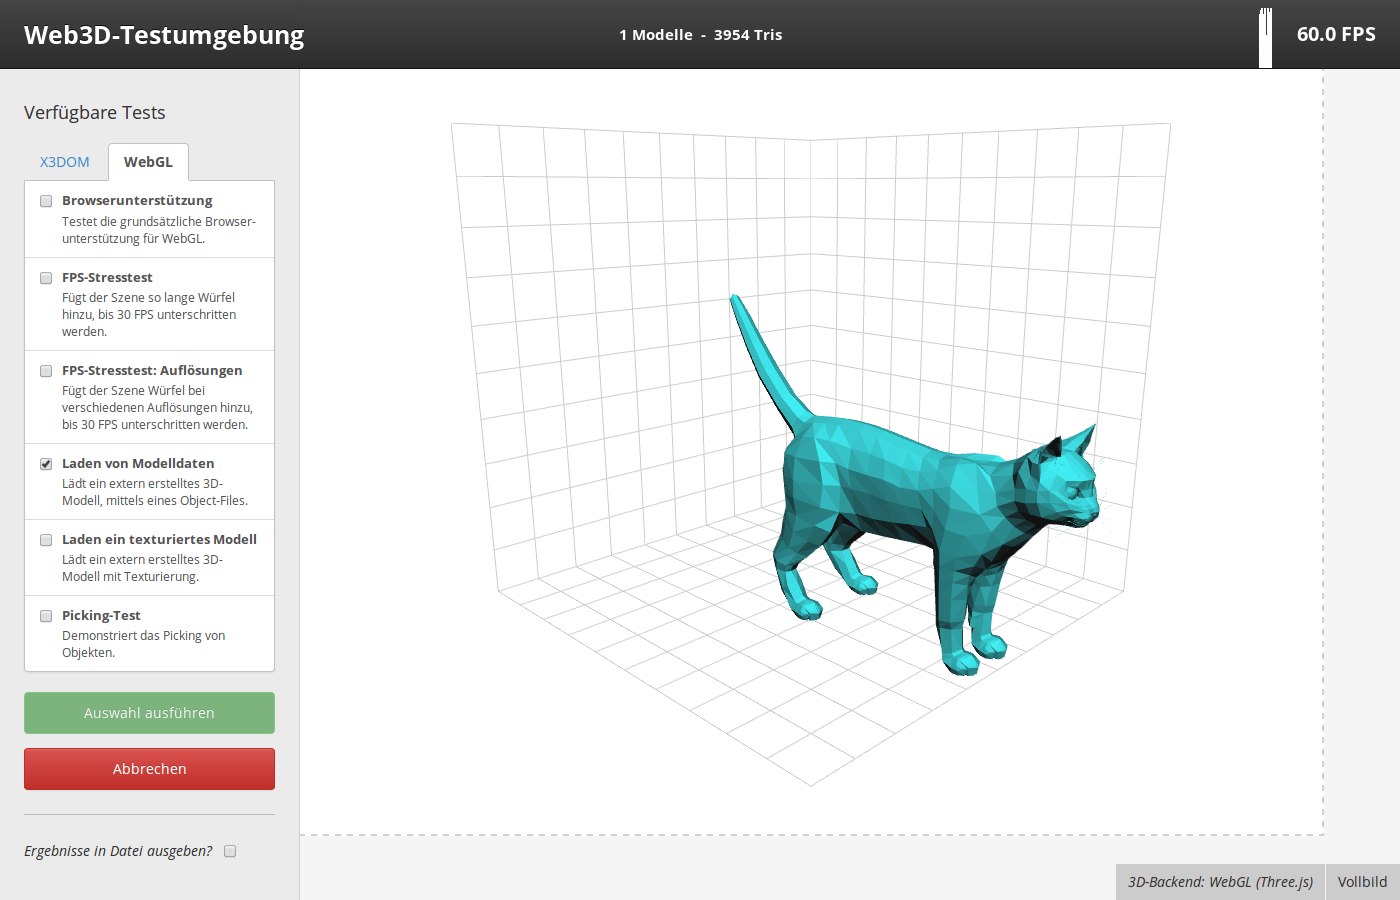
\includegraphics[width=0.48\textwidth]{kap5/figures/test-env-in-action-1.png}
		\label{FIG:WEB3D_TEST_ENV_LOAD_3D_MODEL}
	}
	\hfill
	\subfloat[FPS-Stresstest]{
		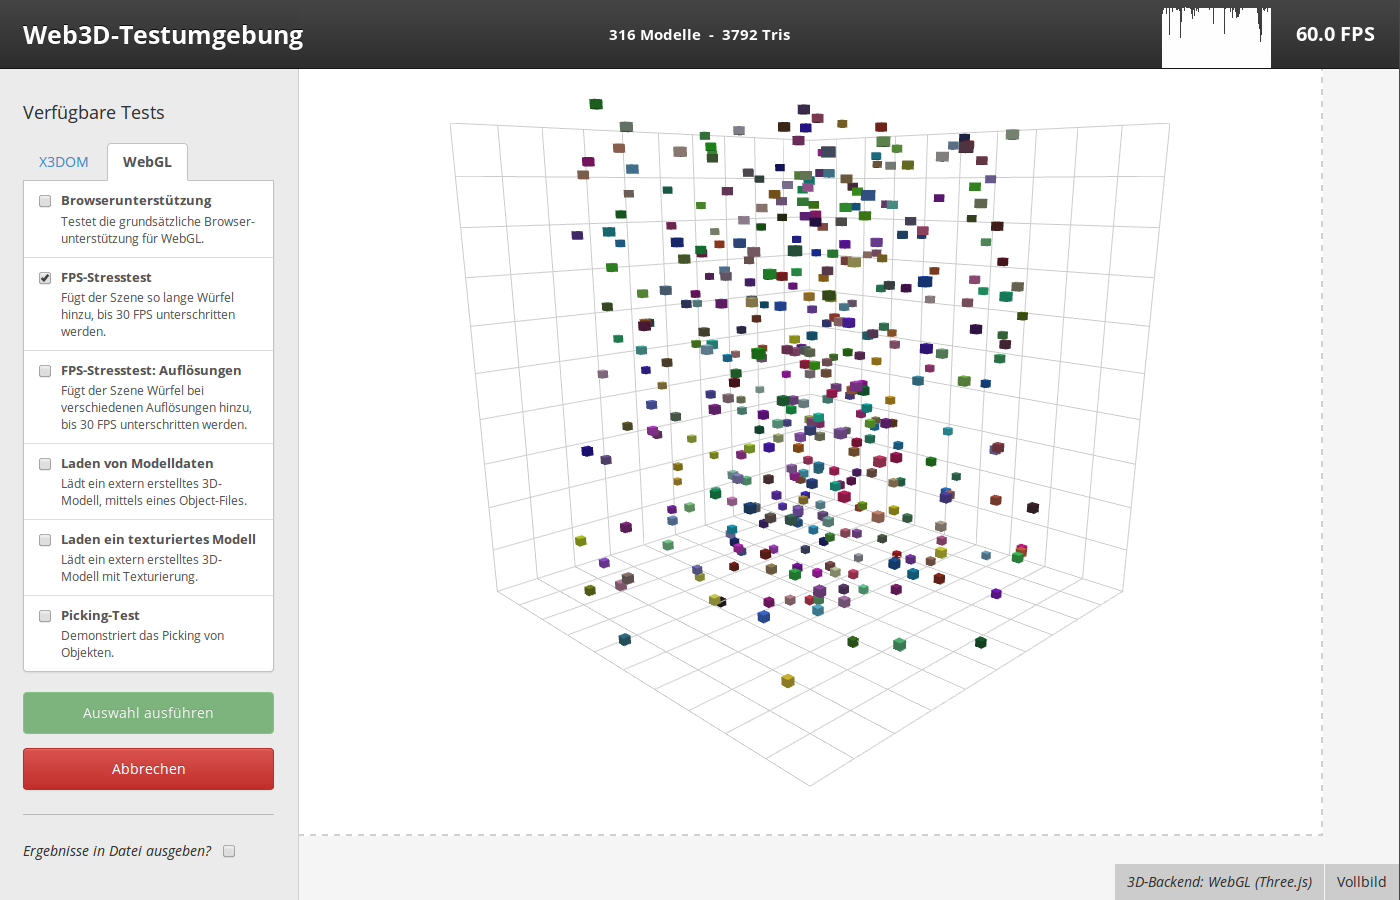
\includegraphics[width=0.48\textwidth]{kap5/figures/test-env-in-action-2.png}
		\label{FIG:WEB3D_TEST_ENV_FPS_STRESSTEST}
	}
	\caption{Verschiedene Tests innerhalb der Testumgebung.}
	\label{FIG:WEB3D_TEST_ENV}
\end{figure}

Zur automatisierten Erprobung von X3DOM und WebGL wurde eine webbasierte Testumgebung umgesetzt, welche die sequentielle Ausführung verschiedener Tests ermöglicht. Die Tests sind auf die spezifizierten Anforderungen zugeschnitten und erproben unterschiedliche Funktionalitäten des Webbrowsers beziehungsweise des Grafiksystems. Abbildung \ref{FIG:TEST_ENV_ARCHITECTURE} zeigt den architektonischen Grundaufbau der Umgebung, die im Folgenden kurz erläutert werden soll.

\begin{figure}[!h]
	\centering
	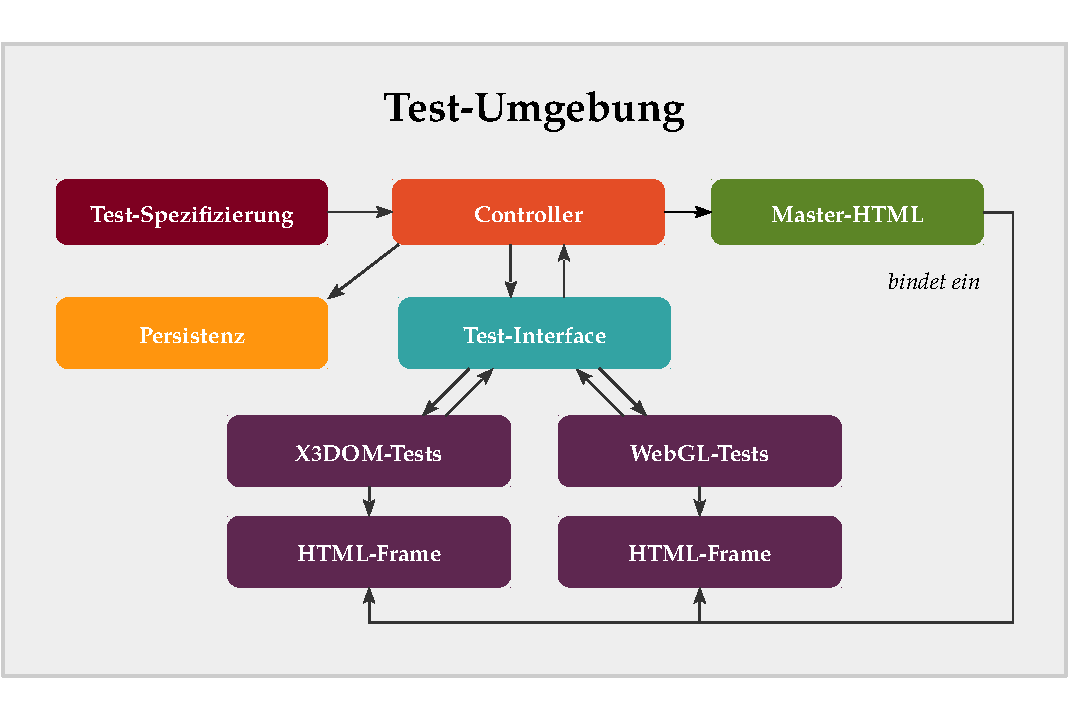
\includegraphics[width=0.8\textwidth]{kap5/figures/test-env-architecture-crop.pdf}
	\caption{Architektur der Testumgebung.}
	\label{FIG:TEST_ENV_ARCHITECTURE}
\end{figure}

Als zentrales Bindeglied der Applikation koordiniert der \emph{Controller} jederzeit den Programmablauf und vermittelt zwischen den einzelnen Komponenten.
Zu Beginn des Ablaufs wird die Test-Spezifikation eingelesen. Diese liegt in Form eines \emph{JSON}-Objekts vor und hat mehrere Funktionen: Zum einen enthält sie die Metadaten der Tests  wie deren textuelle Beschreibung, und zum anderen werden die verschiedenen Testfälle mit einer zugehörigen Funktion verknüpft. Weiterhin werden hier die variierenden Parameter für den späteren Aufruf dieser Methode definiert.

Zur Darstellung der aktuell betrachteten 3D-Technologie dient ein sogenannter \emph{iFrame}. Dieses HTML-""Element ermöglicht das Einbetten eines externen HTML-Dokuments innerhalb eines rechteckigen Rahmens auf einer Webseite. Die so geladene HTML-Seite besitzt ein eigenes \emph{Document Object Model} und operiert größtenteils unabhängig zum Eltern-Dokument. Diese Abschottung hat den Vorteil, dass die 3D-Darstellung innerhalb des \emph{iFrames} in seiner Ausführung durch die Benutzeroberfläche der Testumgebung nicht gestört wird. Darüber hinaus kann das angezeigte HTML-Dokument jederzeit dynamisch durch den Controller mit einem anderen ausgetauscht werden. Dies erleichtert das Testen sowohl von X3D als auch von WebGL in jeweils eigenen Dateien.

Auch die Ausführung der Tests wird vom Controller überwacht. Dieser baut nach der Auswahl der auszuführenden Tests durch den Benutzer eine entsprechende Warteschlange auf und führt die Tests der Reihe nach aus.
Diese sind gegen ein abstrahiertes Test-Interface programmiert und somit unabhängig von ihrer konkreten Implementierung. Für jede der Technologien existiert ein klassenähnliches JavaScript-Objekt, das alle abstrakten Methoden des Test-Interface auf das entsprechende 3D-Framework zugeschnitten, realisiert. Auch das eigentliche Rendern der Szene wird hier umgesetzt.

Um die Messergebnisse der Tests schließlich dauerhaft zu speichern, interagiert der Controller nach Abschluss aller Tests mit der Persistenz-Komponente. Diese dient der Speicherung der volatilen JavaScript-Arrays in einer JSON-Datei, welche daraufhin heruntergeladen werden kann.

\section{Methodik und Testdurchführung}

\subsection{Browserunterstützung und Plattformunabhängigkeit}

Durch das in Abschnitt \ref{SEC:X3D_ARCHITECTURE} beschriebene Fallback-Systems X3DOMs ist ein Test der Browserunterstützung für diese Technologie sehr einfach zu realisieren. Mit dem sogenannten Runtime-Objekt stellt X3DOM eine Schnittstelle zur dynamischen Ansteuerung des Systems bereit. Die Funktion \texttt{backendName} der API liefert den Namen des verwendeten Backends. Falls das Runtime-Objekt nicht existiert, kann X3DOM nicht initialisiert werden, weil keinerlei 3D-Backend zur Verfügung steht. In diesem Fall ist eine 3D-Darstellung durch X3DOM nicht möglich.

\smallskip
\begin{listing}[!htb]
\jsgginput[firstline=146, lastline=150, firstnumber=146]{web3d/tests/x3dom/frame.js}
\caption{Browser-Support-Test für X3DOM.}
\label{LISTING:EVAL_BROWSER_SUPPORT_X3DOM}
\end{listing}

Auch die Überprüfung WebGLs ist leicht zu realisieren. Zunächst wird innerhalb von JavaScript das \texttt{window}-Objekt betrachtet. Dieses stellt das Fenster des Browsers dar und beinhaltet zusätzlich zu dessen Eigenschaften zahlreiche globale Variablen und Schnittstellen zu JavaScript-basierten Webtechnologien. Es wird überprüft, ob \texttt{window} das \texttt{WebGLRenderingContext}-Objekt enthält (vgl. Listing \ref{LISTING:EVAL_BROWSER_SUPPORT_WEBG}, Zeile 170 f.). Wenn dieses Element nicht existiert, ist WebGL in diesem Browser nicht implementiert und es besteht keinerlei Unterstützung für die Technologie. Andernfalls wird versucht den WebGL-Kontext mittels eines dynamisch erstellten Canvas-Elements auszulesen (Zeile 173 ff.). Falls dies fehlschlägt, so ist anzunehmen dass der Webbrowser zwar eine grundsätzliche Unterstützung für WebGL besitzt, aber die Technologie Browser-intern deaktiviert ist.

\smallskip
\begin{listing}[!htb]
\jsgginput[firstline=208, lastline=222, firstnumber=208]{web3d/tests/webgl/frame.js}
\caption{Browser-Support-Test für WebGL.}
\label{LISTING:EVAL_BROWSER_SUPPORT_WEBG}
\end{listing}

Ursache hierfür kann ein instabiler Grafiktreiber beziehungsweise zu schwache Hardware sein. Der Browser unterbindet die Ausführung von WebGL dann anhand einer durch den Hersteller verwalteten \emph{Blacklist}. Die Blacklist beinhaltet Hardwarekomponenten, die dafür bekannt sind, Probleme zu verursachen. Viele Browser erlauben jedoch das explizite Überschreiben dieser internen Deaktivierung WebGLs durch das Setzen sogenannter \emph{Flags} in speziellen Einstellungsdialogen. In Chrome steht dieser beispielsweise bei Eingabe der Adresse \enquote{\texttt{about:flags}} zur Verfügung. In einigen Browser-Versionen ist WebGL darüber hinaus standardmäßig deaktiviert, da die Technologie durch den Hersteller als noch zu experimentell erachtet wird.

Tabelle \ref{TAB_BROWSER_SUPPORT} auf der nächsten Seite zeigt die Testergebnisse dieser Überprüfung auf den betrachteten Plattformen. Wie in der Anforderungsanalyse spezifiziert, wurden hierbei die gängigen Desktop-Betriebsysteme (Windows, Mac OS X und GNU/Linux) untersucht. Weiterhin wurde die Unterstützung innerhalb der mobilen Plattformen Android 4.4 und der aktuellen und zukünftigen Version von iOS getestet (Version 7 und 8).

\begin{table}[tbp]
	\centering
	\small
	\begin{tabularx}{\textwidth}{llYYYYYYY}
		\toprule
						& Gerät
						& \footnotesize 
\includegraphics[height=1em]{kap5/figures/chrome.eps}\hspace{1ex}\textsf{36}
						& \footnotesize 
\includegraphics[height=1em]{kap5/figures/firefox.eps}\hspace{1ex}\textsf{31}
						& \footnotesize 
\includegraphics[height=1em]{kap5/figures/ie.eps}\hspace{1ex}\textsf{9}
						& \footnotesize 
\includegraphics[height=1em]{kap5/figures/ie.eps}\hspace{1ex}\textsf{10}
						& \footnotesize 
\includegraphics[height=1em]{kap5/figures/ie.eps}\hspace{1ex}\textsf{11}
						& \footnotesize 
\includegraphics[height=1em]{kap5/figures/opera.eps}\hspace{1ex}\textsf{23}\textsuperscript{*}
						& \footnotesize 
\includegraphics[height=1em]{kap5/figures/safari.eps}\hspace{1ex}\textsf{7} \\
		\midrule
		\small
		Windows 7		& Desktop
						& \xpie{2} \wpie{1}
						& \xpie{2} \wpie{1}
						& \xpie{1} \wpie{0}
						& \xpie{1} \wpie{0}
						& \xpie{2} \wpie{1}
						& \xpie{2} \wpie{1}
						& - 					\\
		Mac OS X 10.9	& Notebook % DONE
						& \xpie{2} \wpie{1}
						& \xpie{2} \wpie{1}
						& --
						& --
						& --
						& \xpie{2} \wpie{1}
						& \xpie{1} \wpie{0}	 	\\
		Ubuntu 14.04	& Desktop
						& \xpie{2} \wpie{1}
						& \xpie{2} \wpie{1}
						& --
						& --
						& --
						& \xpie{2} \wpie{0.5}
						& -- 					\\
		Arch Linux		& Desktop %DONE
						& \xpie{2} \wpie{1}
						& \xpie{2} \wpie{1}
						& --
						& --
						& --
						& \xpie{2} \wpie{0.5}
						& -- 					\\
		Android 4.4 	& Nexus 7 % DONE
						& \xpie{2} \wpie{1}
						& \xpie{2} \wpie{1}
						& --
						& --
						& --
						& \xpie{2} \wpie{1}
						& --          			\\
		iOS 7			& iPad 3 % DONE
						& \xpie{0} \wpie{0}
						& --
						& --
						& --
						& --
						& --
						& \xpie{0} \wpie{0} 	\\
		iOS 8 (\emph{Beta})	& Simulator % DONE
						& \xpie{2} \wpie{1}
						& --
						& --
						& --
						& --
						& --
						& \xpie{2} \wpie{1} 	\\
		Android 4.4 	& Nexus 5 % DONE
						& \xpie{2} \wpie{1}
						& \xpie{2} \wpie{1}
						& --
						& --
						& --
						& \xpie{2} \wpie{1}
						& --          			\\
		iOS 7			& iPhone 5s
						& \xpie{0} \wpie{0}
						& --
						& --
						& --
						& --
						& --
						& \xpie{0} \wpie{0}		\\
		\bottomrule
	\end{tabularx}
	\begin{minipage}{0.25\linewidth}%
		\vspace{1ex}
		\begin{itemize}[leftmargin=*,label={}]
			\scriptsize
			\itemsep0em
			\item\tikz \fill [x3domc] (0.1,0.1) rectangle (0.25,0.25);\hspace{1.5ex}X3DOM
			\item\tikz \fill [webglc] (0.1,0.1) rectangle (0.25,0.25);\hspace{1.5ex}WebGL
			\item\small--\scriptsize\hspace{1.5ex}Browser nicht verfügbar
		\end{itemize}
	\end{minipage}%
	\begin{minipage}{0.25\linewidth}%
		\vspace{1ex}
		\begin{itemize}[leftmargin=*,label={}]
			\scriptsize
			\itemsep0em
			\item\small\xpie{0}\scriptsize\hspace{1.5ex}Keine Unterstützung
			\item\small\xpie{1}\scriptsize\hspace{1.5ex}Flash-Backend
			\item\small\xpie{2}\scriptsize\hspace{1.5ex}WebGL-Backend
		\end{itemize}
	\end{minipage}%
	\begin{minipage}{0.25\linewidth}%
		\vspace{1ex}
		\begin{itemize}[label={}]
			\scriptsize
			\itemsep0em
			\item\small\xpie{3}\scriptsize\hspace{1.5ex}X3D-Plugin
			\item\small\xpie{4}\scriptsize\hspace{1.5ex}Natives X3D
			\item%
		\end{itemize}
	\end{minipage}%
	\begin{minipage}{0.25\linewidth}%
		\vspace{1ex}
		\begin{itemize}[leftmargin=*,label={}]
			\scriptsize
			\itemsep0em
			\item\small\wpie{0}\scriptsize\hspace{1.5ex}Keine Unterstützung
			\item\small\wpie{0.5}\scriptsize\hspace{1.5ex}Teilweise unterstützt
			\item\small\wpie{1}\scriptsize\hspace{1.5ex}Unterstützt
		\end{itemize}
	\end{minipage}%
	\vspace{0.5ex}%
	\center\scriptsize * Anmerkung: Opera unter GNU/Linux in Version 12.
	\vspace{0.5ex}%
	\caption{Unterstützung von X3DOM und WebGL auf verschiedenen Testsystemen.}
	\label{TAB_BROWSER_SUPPORT}
\end{table}

In den meisten Testfällen zeigt sich ein einheitliches Bild: WebGL wird auf fast allen Plattformen nativ unterstützt. Dadurch ist eine Darstellung von X3D durch X3DOM mit entsprechendem Backend möglich. Eine Ausnahme stellt die derzeitige Version 7 von iOS dar: Der Standard-Browser Safari von Apple bietet weder für X3DOM noch für WebGL eine Unterstützung. Aufgrund der fehlenden Unterstützung von iOS für Adobe Flash steht auch dieses Fallback-Model nicht zur Verfügung.
Interessanterweise besteht bereits seit iOS 5 eine Implementierung WebGLs in Safari. Diese ist jedoch abgesehen von der Werbeplattform \emph{iAd} deaktiviert und kann nicht angesprochen werden \autocite{Benin:2012:THM:2338714.2338734}. Wie bereits im Motivationsteil erwähnt, wird mit der Veröffentlichung von iOS 8 jedoch auch dieses Hinderniss durch die Aktivierung WebGLs überwunden sein \autocite{APPLE_WWDC_2014_WEBGL}.
Auch in der Desktop-Variante von Safari unter Mac OS X ist WebGL bis dato nicht verfügbar. Es ist jedoch davon auszugehen, dass WebGL ähnlich zu iOS mit der für Herbst 2014 angesetzten Version 8 von Safari aktiviert sein wird. Sofern das Flash-Plugin installiert ist, bietet der Browser derzeit zumindest eine X3DOM-Unterstützung durch das Flash-Backend.

Ebenso aus dem Raster fallen die Linux-Vertreter Ubuntu 14.04 und Arch Linux. Unter GNU/Linux liegt Opera noch in Version 12 vor und hinkt der aktuellen Versionsnummer 23 nach. Die Ursache für diesen Unterschied ist die 2013 vollzogenen Umstrukturierung des Browsers. Nach einem Wechsel zur HTML-Rendering-Engine \emph{Blink}, einer Abspaltung von \emph{Webkit}, wurde Opera auf Basis von Chromium\footnote{Chromium ist das Open-Source-Projekt hinter Googles Webbrowser Chrome.} neu aufgesetzt \autocite{OPERA_SWITCHES_TO_WEBKIT}. Zwar existiert in Opera 12 eine WebGL-Implementierung, sie ist jedoch standardmäßig deaktiviert und muss durch die oben beschriebene \emph{Flag} im Browser explizit aktiviert werden.

Da WebGL erst ab Internet Explorer 11 unterstützt wird, steht in den Versionen 9 und 10 lediglich bei X3DOM eine Unterstützung für 3D-Darstellung zu Verfügung, wenn ein Flash-Plugin installiert ist.

\subsection{Vergleich der Hardware-Anforderungen}

Um die Hardware-Anforderungen und die Performance der zwei Technologien gegenüberzustellen, wurde innerhalb der Testumgebung ein GPU-Stress-Test implementiert. Hierbei werden der 3D-""Szene so lange Würfel hinzugefügt, bis die Bildwiederholrate (\emph{Framerate}) wie in Abschnitt \ref{SECTION:HARDWARE_REQUIREMENTS} spezifiziert unter 25 Bilder pro Sekunde (\emph{FPS}) fällt. Die Zahl der grafischen Primitive und der Polygone (Dreiecke) wird dabei mit aufgezeichnet. Um eine Vergleichbarkeit der Betriebsysteme zu gewährleisten, wurde der Test auf allen Plattformen in Google Chrome ausgeführt.

\begin{figure}[p]
	\centering
	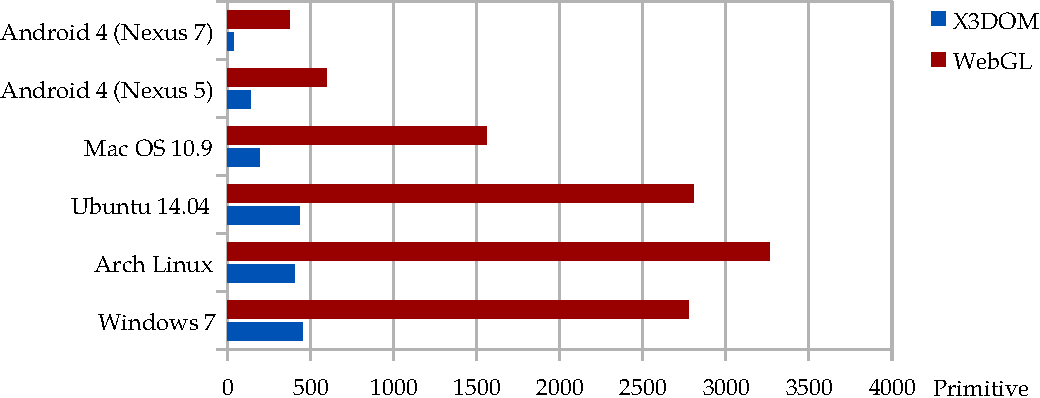
\includegraphics[width=0.9\textwidth]{kap5/figures/test-fps-all-os-chrome-crop.pdf}
	\vspace{0.75ex}
	\caption{FPS-Stresstest für 25 FPS in Google Chrome.}
	\label{FIG:GEOMETRY_TEST_CHROME}
\end{figure}

\begin{figure}[p]
	\centering
	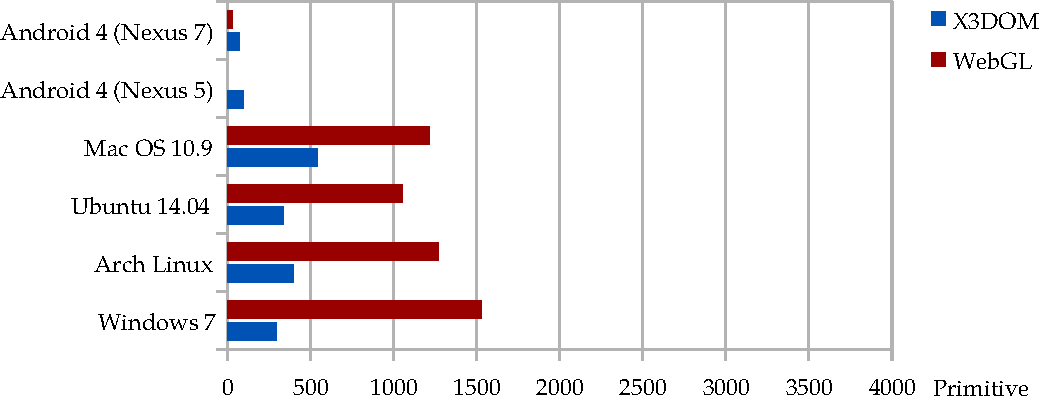
\includegraphics[width=0.9\textwidth]{kap5/figures/test-fps-all-os-ff-crop.pdf}
	\vspace{0.75ex}
	\caption{FPS-Stresstest für 25 FPS in Firefox.}
	\label{FIG:GEOMETRY_TEST_FIREFOXL}
\end{figure}

\begin{figure}[p]
	\centering
	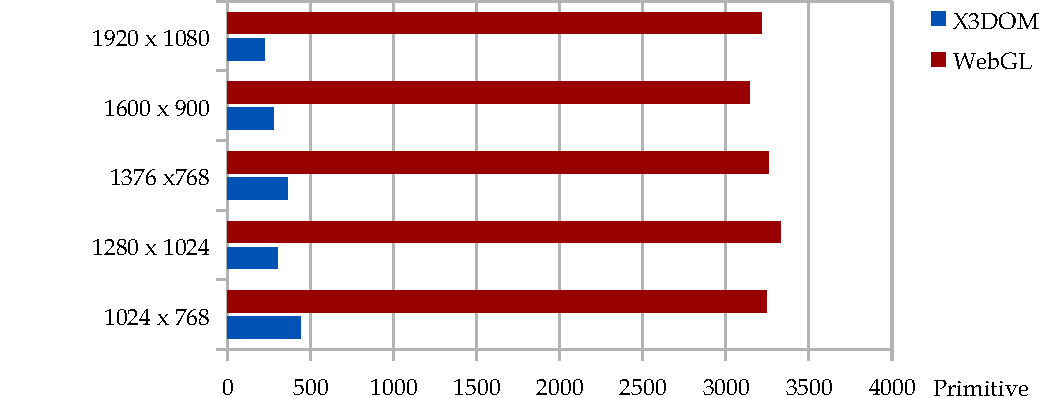
\includegraphics[width=0.9\textwidth]{kap5/figures/test-fps-all-res-chrome-crop.pdf}
	\vspace{0.75ex}
	\caption{FPS-Stresstest für verschiedene Auflösungen.}
	\label{FIG:GEOMETRY_RESOLUTION_TEST_CHROME}
\end{figure}

Die Messergebnisse in Abbildung \ref{FIG:GEOMETRY_TEST_CHROME} auf der nächsten Seite zeigen eine enorme Differenz zwischen X3DOM und WebGL auf. WebGL schafft im Test unter Chrome auf jeder Plattform im Schnitt über sieben mal mehr Primitive als X3DOM darzustellen, ehe die Framerate unter 25 Bilder pro Sekunde fällt.

Da X3DOM in allen betrachteten Fällen das WebGL-Backend und damit die gleiche Technologie für das Rendering verwendete, ist dieses Ergebnis überraschend.
Die Vermutung dass dieser deutlich schlechtere Wert auf die große Zahl von teuren DOM-Manipulationen durch X3DOM zurückzuführen ist, hat sich nicht bestätigt. Auch für verhältnismäßig große Zeitintervalle wie 1000 Millisekunden zwischen dem Hinzufügen eines weiteren Würfels bleiben die erzielten Werte etwa gleich. Der Grund für diesen Unterschied scheint daher in der grundsätzlichen Architektur der zwei Ansätze zu liegen. Die in Abschnitt \ref{SEC:X3D_ARCHITECTURE} erörterte Zustandssynchronisierung der X3D-Knoten im DOM des HTML-Dokuments mit dem X3D-Backend führt wahrscheinlich zu einem größeren Rechenaufwand pro Einzelbild, als ihn Three.js als relativ schlanke Abstraktionsschicht zu WebGL verursacht.

Zum Vergleich der verschiedenen Webbrowser werden die Ergebnisse des Stress-Tests auch für Firefox in Abbildung \ref{FIG:GEOMETRY_TEST_FIREFOXL} gezeigt. Während die X3DOM-Werte in etwa gleich bleiben, liegt die Performance von WebGL bei Firefox klar hinter der bei Google Chrome gemessenen. Weiterhin können bei WebGL mehr als zwei mal so viel Geometrien dargestellt werden als bei X3DOM, ehe die FPS-Untergrenze erreicht ist.
Der Unterschied zu Google Chrome verdeutlicht die Varianz der Leistungsfähigkeit der WebGL-Implementierungen in den verschiedenen Browsern. Auch die Performance der jeweiligen JavaScript-Engine ist hierbei relevant, da sie beispielsweise die Geschwindigkeit von DOM-Manipulationen direkt beeinflusst.

Der Stress-Test für 25 Frames wurde zudem bei verschiedenen Bildschirmauflösungen durchgeführt, um deren Einfluss auf die Bildwiederholfrequenz zu untersuchen. Die Auflösung wird durch dynamisches Setzen der \emph{iFrame}-Größe simuliert. Um das Ergebnis nicht durch Clipping zu verfälschen, wird der Test im Vollbild-Modus durchgeführt. Der Bildschirm des Testsystems muss dabei die maximale Auflösung von 1920 x 1080 Pixeln unterstützen. Abbildung \ref{FIG:GEOMETRY_RESOLUTION_TEST_CHROME} auf der vorhergehenden Seite zeigt die gemessenen Ergebnisse.
% TODO: Abchecken

Die Zahl der darstellbaren Geometrien bleibt für jede der untersuchten Auflösungen wider Erwarten sowohl für X3DOM als auch für WebGL auf fast gleichem Niveau. Eine mögliche Erklärung für dieses Ergebniss könnte in JavaScript liegen. Zwar hat die Performance heutiger JavaScript-Engines innerhalb der letzten Jahre stark zugenommen \autocite{Evans201443}, dennoch liegt diese aufgrund der dynamischen Natur von JavaScript weit hinter klassisch kompilierten Sprachen wie C++. Des Weiteren führen die insbesondere bei X3DOM häufigen DOM-Manipulationen zu einem möglichen Flaschenhals.

\subsection{Import von 3D-Modellen}

Der nächste Test behandelt das Laden eines extern erstellten 3D-Modells. Beide Technologien unterstützen diese Anforderung. Das Vorgehen bei X3DOM und WebGL unterscheidet sich dabei jedoch in der Komplexität, wie nachfolgend ausgeführt werden soll.

X3D ermöglicht es, mittels des \texttt{Inline}-Knotens sehr einfach eine externe X3D-Datei einzubinden. Hierdurch wird dem aktuellen Szenengraph an dieser Stelle der Inhalt dieser Datei angefügt, sodass ein Subszenengraph entsteht. Das Framework lädt die Daten automatisch mittels asynchroner HTTP-Anfragen. Hierdurch wird das Laden der 3D-Darstellung nicht blockiert, sondern die Elemente der Szene dynamisch nach und nach hinzugefügt, sobald sie zur Verfügung stehen.

\smallskip
\begin{listing}[ht]
\begin{htmlcode}
<Scene>
	<!-- Weitere Elemente -->
	<Transform>
          <Inline url='model.x3d'></Inline>
    </Transform>
<Scene>
\end{htmlcode}
\caption{Einbinden einer X3D-Datei in X3DOM.}
\label{LISTING:X3DOM_INLINE_NODE}
\end{listing}

Die X3D-Dateien können beispielsweise mit der freien 3D-Modellierungssoftware Blender \autocite{SOFTWARE_BLENDER} erstellt werden. Blender ermöglicht den Import einer Vielzahl verschiedener 3D-Formate und kann das Modell im Anschluss in eine X3D-Datei exportieren, welche wie gezeigt in X3DOM direkt eingebunden werden kann.

Das Laden eines 3D-Modells in WebGL wird durch Three.js vereinfacht, indem dieses einige zusätzliche Hilfsmodule für verschiedene 3D-Formate mitliefert. Ein einfaches, häufig verwendetes Format ist das \emph{Wavefront OBJ Format}. Dieses spezifiziert die \emph{Vertices}, Seiten und Normalen und optional die Texturkoordinaten (\emph{Texture Mapping}) eines Polygons.
Three.js stellt für dieses Format einen Mechanismus bereit, um den Inhalt der Datei asynchron zu laden und wandelt das enthaltene Modell direkt in eine Framework-eigene Datenstruktur um. Die so geladene Geometrie kann der Szene anschließend hinzugefügt werden.

\subsection{Benutzerinteraktion}

\subsubsection{Navigation}

Sowohl in X3DOM als auch in Three.js stehen einige vorgefertige Navigations-Modi bereit, die es dem Benutzer erlauben, sich auf verschiedene Arten durch die 3D-Welt zu bewegen. Innerhalb der Testumgebung wird bei jedem Test eine in der Anforderungsanalyse beschriebene Orbit-Navigation verwendet. Hierdurch kann die Darstellung beliebig gedreht, verschoben und skaliert werden.

\smallskip
\begin{listing}[!h]
\begin{htmlcode}
<Scene>
	<NavigationInfo type='examine'></NavigationInfo>
	<!-- Weitere Elemente -->
<Scene>
\end{htmlcode}
\caption{Setzen des Navigations-Modus in X3DOM.}
\label{LISTING:X3DOM_NAVIGATION_INFO_NODE}
\end{listing}

Der Navigationsmodus wird in X3DOM mittels des \texttt{NavigationInfo}-Knoten ausgewählt und kann mit JavaScript jederzeit dynamisch verändert werden (vgl. Listing \ref{LISTING:X3DOM_NAVIGATION_INFO_NODE}. Da viele der Modi lediglich geringfügige Abwandlungen einer anderen Navigationstechnik sind, werden hier nur die wichtigsten kurz umrissen: Die Option \emph{Examine} entspricht der Orbit-Navigation. Weiterhin stehen \emph{Fly} und \emph{Walk} zur Verfügung. Während \emph{Fly} eine völlig freie Bewegung im Raum zulässt, ist der Benutzer bei \emph{Walk} hinsichtlich der Y-Achse auf den Untergrund eingeschränkt. Schließlich unterstützt das Framework den Modus \emph{Look at}. Hierbei bewegt sich die Kamera in Richtung eines durch Klick anvisierten Punktes im Raum, sodass dieser näher betrachtet werden kann.

Auch Three.js stellt durch die beigefügten Beispiele des Frameworks einige Navigationstechniken bereit, die den Modi von X3DOM sehr ähnlich sind. Die Hilfsmodule sind zwar kein offizieller Bestandteil des Frameworks, funktionieren jedoch zuverlässig. Zu den wichtigsten gehören die Orbit-Navigation, ein Flugmodus und eine Bewegung in der Art eines \emph{First Person Shooters}.

\subsubsection{Auswahl von Objekten (Picking)}

Ein weiterer wichtiger Punkt der Benutzerintaktion ist das Auswählen einzelner 3D-Objekte im Raum, um eine zugehörige Aktion wie beispielsweise die Anzeige eines Popups auszulösen. Hierbei wird ein sogenanntes \emph{Picking}-Verfahren angewandt. Picking kehrt die Projektion der 3D-Darstellung auf den zweidimensionalen Bildschirm um, indem ein Lichtstrahl ausgehend von der Klickposition in Blickrichtung der Kamera ausgesendet wird \autocite{THREEJS_PICKING}. Sobald der Strahl auf ein Objekt trifft, gilt dieses als angeklickt.

In X3DOM ist dieses Verfahren bereits integriert und äußerst einfach in der Anwendung. Einem Shape-Knoten kann mittels des Attributs \texttt{onClick} analog zu klassischem HTML eine aufzurufende Funktion (\emph{Event-Handler}) zugewiesen oder ein JavaScript-Ausdruck direkt eingebettet werden:

\smallskip
\begin{listing}[ht]
\begin{htmlcode}
<Shape>
	<Appearance>
		<Material diffuseColor='1 0 0'></Material>
	</Appearance>
	<Box onclick='clickHandler(event)'></Box>
</Shape>
\end{htmlcode}
\caption{Deklaration eines \emph{onclick-Handlers} in X3DOM.}
\label{LISTING:X3DOM_ONCLICK_HANDLER}
\end{listing}

Bei WebGL ist eine Umsetzung von Picking komplizierter. Three.js vereinfacht die Implementierung dabei aber erheblich durch Bereitstellung einiger Hilfsmethoden. Mittels des \texttt{Projector}-Objekts des Frameworks kann der Strahlengang nach einem Mausklick im Raum verfolgt werden und ermöglicht so die Ermittlung der Objekte unterhalb des Mauszeigers. Diese können im Anschluss beliebig manipuliert werden. Im Test werden die zur Demonstration eingefügten Würfel beim Überfahren mit der Maus schwarz eingefärbt und verschwinden, sobald auf sie geklickt wird.

\subsection{Realistische Grafikdarstellung}

Für die realistische Darstellung von 3D-Modellen ist, wie in der Anforderungsanalyse ausgeführt, insbesondere die Beleuchtung, der Schattenwurf, das Shading und die Texturierung entscheidend. Der Realismus-Test demonstriert diese Aspekte durch eine entsprechende Darstellung der Utah-Teekanne\footnote{Die Utah-Teekanne wurde 1975 von dem Computergrafiker Martin Newell im Rahmen einer Forschungsarbeit an der Universität von Utah entworfen. Sie hat sich zu einer Art \enquote{\em{Hello Word}} der Computergrafik entwickelt und dient sehr häufig als beispielhaftes 3D-Modell \autocite{UTAH_TEAPOT}.} durch X3DOM und Three.js.

\begin{figure}[!h]
	\centering
	\subfloat[X3DOM (WebGL-Backend)]{
		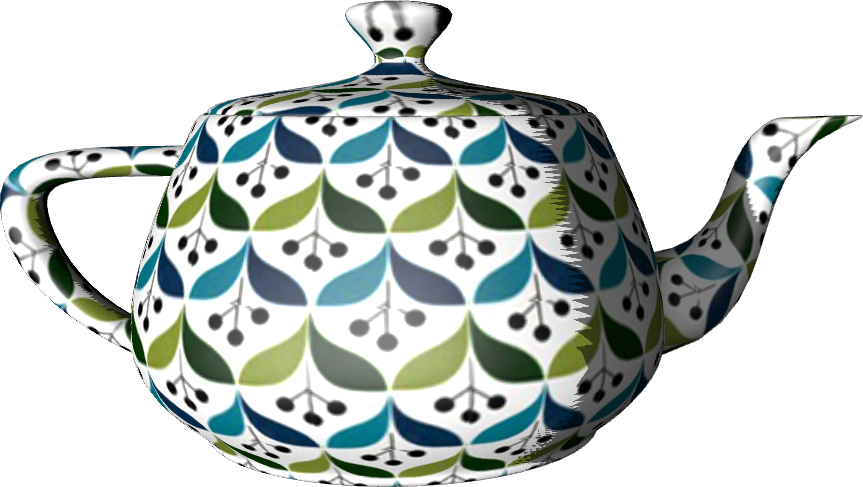
\includegraphics[width=0.48\textwidth]{kap5/figures/realism-x3dom.png}
		\label{FIG:REALISM_TEST_X3DOM}
	}
	\hfill
	\subfloat[WebGL]{
		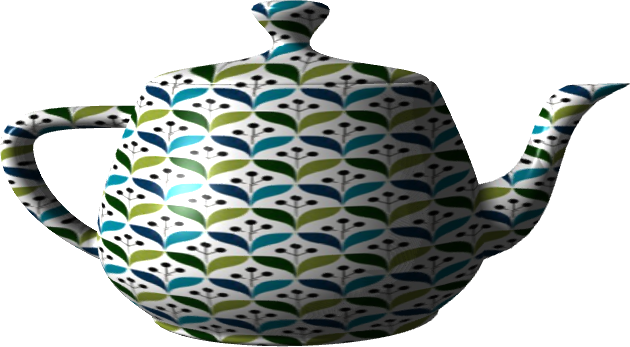
\includegraphics[width=0.48\textwidth]{kap5/figures/realism-webgl.png}
		\label{FIG:REALISM_TEST_WEBGL}
	}
	\caption{Vergleich der texturierten 3D-Modelle.}
	\label{FIG:REALISM_TEST}
\end{figure}

Abbildung \ref{FIG:REALISM_TEST} zeigt das jeweilige Resultat des mit einem Muster texturierten 3D-Modells. Beide Frameworks unterstützen Smooth-Shading mit einer diffusen und spekularen Reflexion. Hierdurch wird eine glatte Oberfläche der Teekane mit Glanzeffekten erzielt. Auch Schatten kann in beiden Ansätzen realisiert werden. Dabei zeigt sich jedoch ein Unterschied hinsichtlich der Qualität der Darstellung. Bei genauer Betrachtung der Schattenkontur in Abbildung \ref{FIG:REALISM_TEST_X3DOM} zeigt sich, anders als bei WebGL, kein weicher Übergang der Schattierung, sondern eine harte, ausgefranste Kante. Generell wirkt das mit Three.js gerenderte 3D-Modell hierdurch visuell ansprechender.

\subsection{Entwicklungs-Aufwand}

Aus den in Anforderung \ref{SEC:DEVELOPMENT_EFFORT} ausgeführten Gründen ist auch der Entwicklungsaufwand ein wichtiger zu bedenkender Faktor für die Umsetzung einer Web3D-Anwendung. Die bisherigen Beispiele und Erläuterungen veranschaulichen gut die paradigmatisch grundverschiedene Vorgehensweise des deklarativen (X3DOM) und des imperativen (WebGL) Vertreters von Web3D.

Während X3D durch den XML-basierten Aufbau eine sehr hohe Konvergenz zu gut verstandenen Webtechnologien wie HTML aufweist, stellt WebGL einen typischen Webentwickler aufgrund des sehr niedrigen Abstraktionsniveaus der Bibliothek vor anspruchsvollere Konzepte \autocite{Jankowski:2013:DII:2466533.2466547}. Die große Nähe zu Open GL ES erfordert ein weitaus tiefgreiferendes Verständis für die theoretischen Grundlagen der Computergrafik, als es X3D durch seinen deklarativen Stil verlangt. Populäre WebGL-Frameworks wie das behandelte Three.js können diese Hürde zwar durch Abstraktion der Funktionalität deutlich senken, dennoch ist der Einarbeitungsaufwand bei WebGL höher einzustufen.

\section{Bewertung der Testergebnisse}

Die Browser- und Plattformunterstützung ist bei beiden Technologien durch das WebGL-Backend von X3DOM sehr ähnlich. Wie Tabelle \ref{TAB_BROWSER_SUPPORT} zeigt, steht WebGL und damit auch X3D in nazu allen aktuellen Browser-Versionen zur Verfügung. Wie ausgeführt besitzt X3DOM ein ausgereiftes Fallback-System und kann bei Bedarf dynamisch auf das weit verbreitete Flash-Plugin umschalten. Hierdurch können auch Benutzer des Internet Explorers 9 und 10 adressiert werden, woraus eine größere generelle Browserunterstützung resultiert. Mit der Veröffentlichung von iOS 8 im Herbst 2014 wird zudem auch eine der letzten verbleibenden Plattformen eine Unterstützung für WebGL erhalten.

Wie der Vergleich der Hardware-Anforderungen zeigt, ist WebGL zumindest innerhalb des betrachteten Testfalls, also bei vielen Geometrien in einer Szene, leistungstechnisch X3DOM überlegen. Bezogen auf die exemplarischen Anwendungsfälle, welche zu Beginn der Anforderungsanalyse in Abschnitt \ref{SEC:APPLICATION_DOMAIN} beschrieben wurden, würde dieser Fall bespielsweise bei der Darstellung komplexer wissenschaftlicher Abbildungen mit sehr vielen Einzelelementen auftreten. Bei Betrachtung eines einzelnen Produkts tritt dieser Aspekt hingegen in den Hintergrund und andere Kriterien wie der Entwicklungsaufwand und die generelle Einfachheit bei der Umsetzung gewinnen an Bedeutung. Hinsichtlich dieser Kriterien ist X3DOM gegenüber WebGL aufgrund seines deklarativen Ansatzes zu bevorzugen. Im Gegensatz zu WebGL, welches ein zumindest grundlegendes Verständnis computergrafischer Konzepte und der Grafik-Pipeline erfordert, sind hier bereits wenige HTML-Kenntnisse ausreichend, um eine 3D-Szene mittels X3DOM umzusetzen.

Beide Frameworks ermöglichen das Importieren einiger offener 3D-Grafikformate, sodass bestehende 3D-Modelle problemlos eingebunden werden können. Dabei ist gegebenfalls eine Umwandlung des Ausgangsmodells in ein durch X3DOM beziehungsweise Three.js unterstütztes Format durch Modellierungssoftware wie Blender \autocite{SOFTWARE_BLENDER} notwendig. Durch die Unterstützung der gängigen Beleuchtungs-Modelle, Shading-Verfahren und Texturierung verhalten sich beide Ansätze hinsichtlich der realistischen Darstellung von 3D-Modellen ähnlich. X3DOM wies innerhalb des Tests hier jedoch einige Artefakte bei der Schattenkontur auf. Die spezifizierten Anforderungen bezüglich der Benutzerinterkation können in beiden Technologien gleich gut realisiert werden.
